\section{Models relevant to Earth-Moon crossings}
\label{sec:appendix}
%\setcounter{page}{1}
%\renewcommand{\thepage}{\thesection -\arabic{page}}

\begin{figure*}[!h] %[!thb]
	\centering
	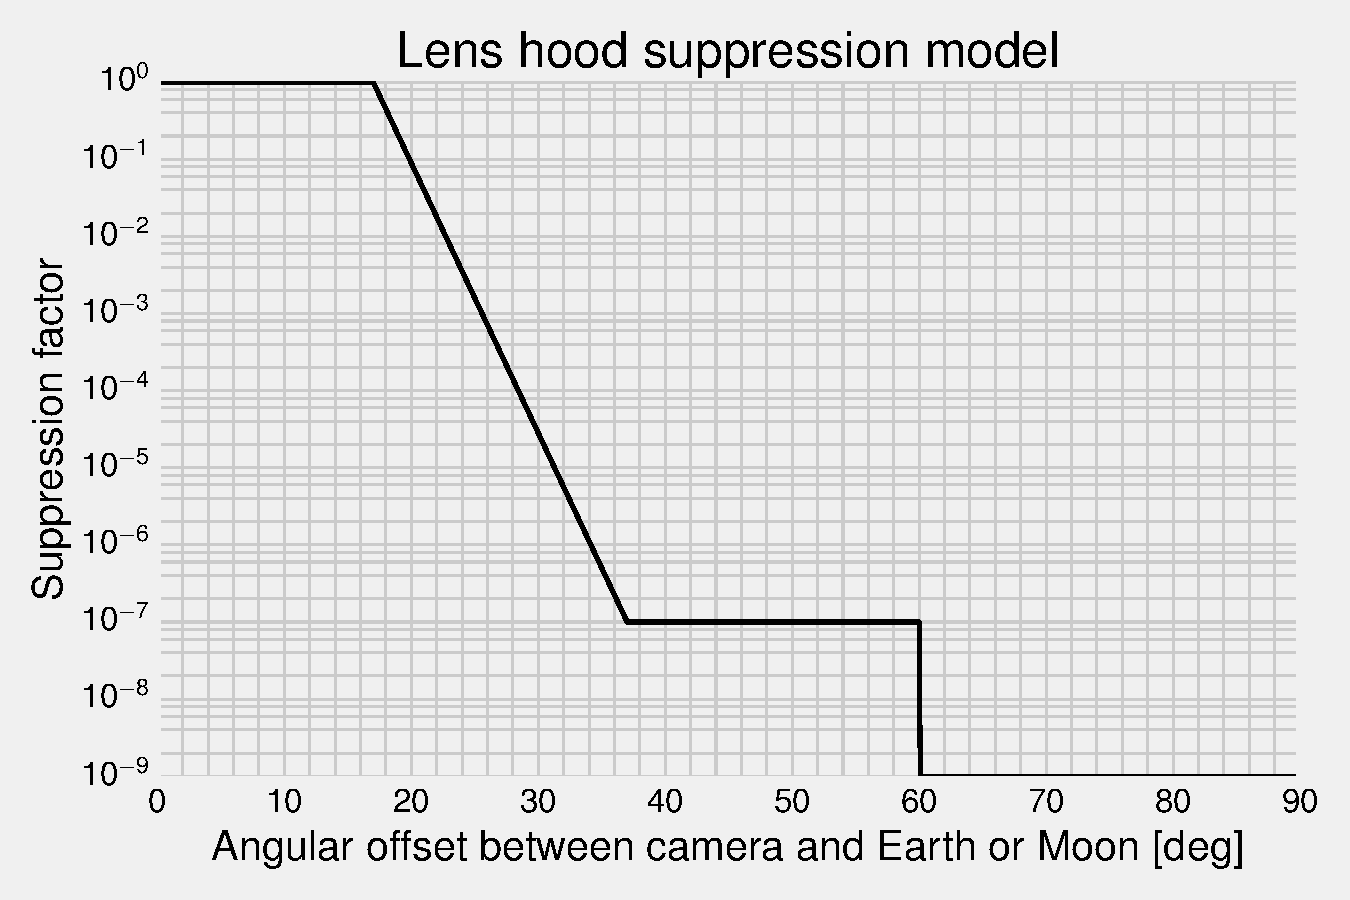
\includegraphics{figures/lens_hood_suppression.pdf}
	%\missingfigure{foobar}	
	\caption{Lens hood suppression plotted against the angular offset to the Earth or Moon. This suppression factor is defined as the fraction of incident flux that is blocked by the spacecraft, sunshade, lens hood, or combinations thereof.}
	\label{fig:lens_hood_suppression}
\end{figure*}
\newpage
\begin{figure*}[!t] %[!thb]
	\centering
	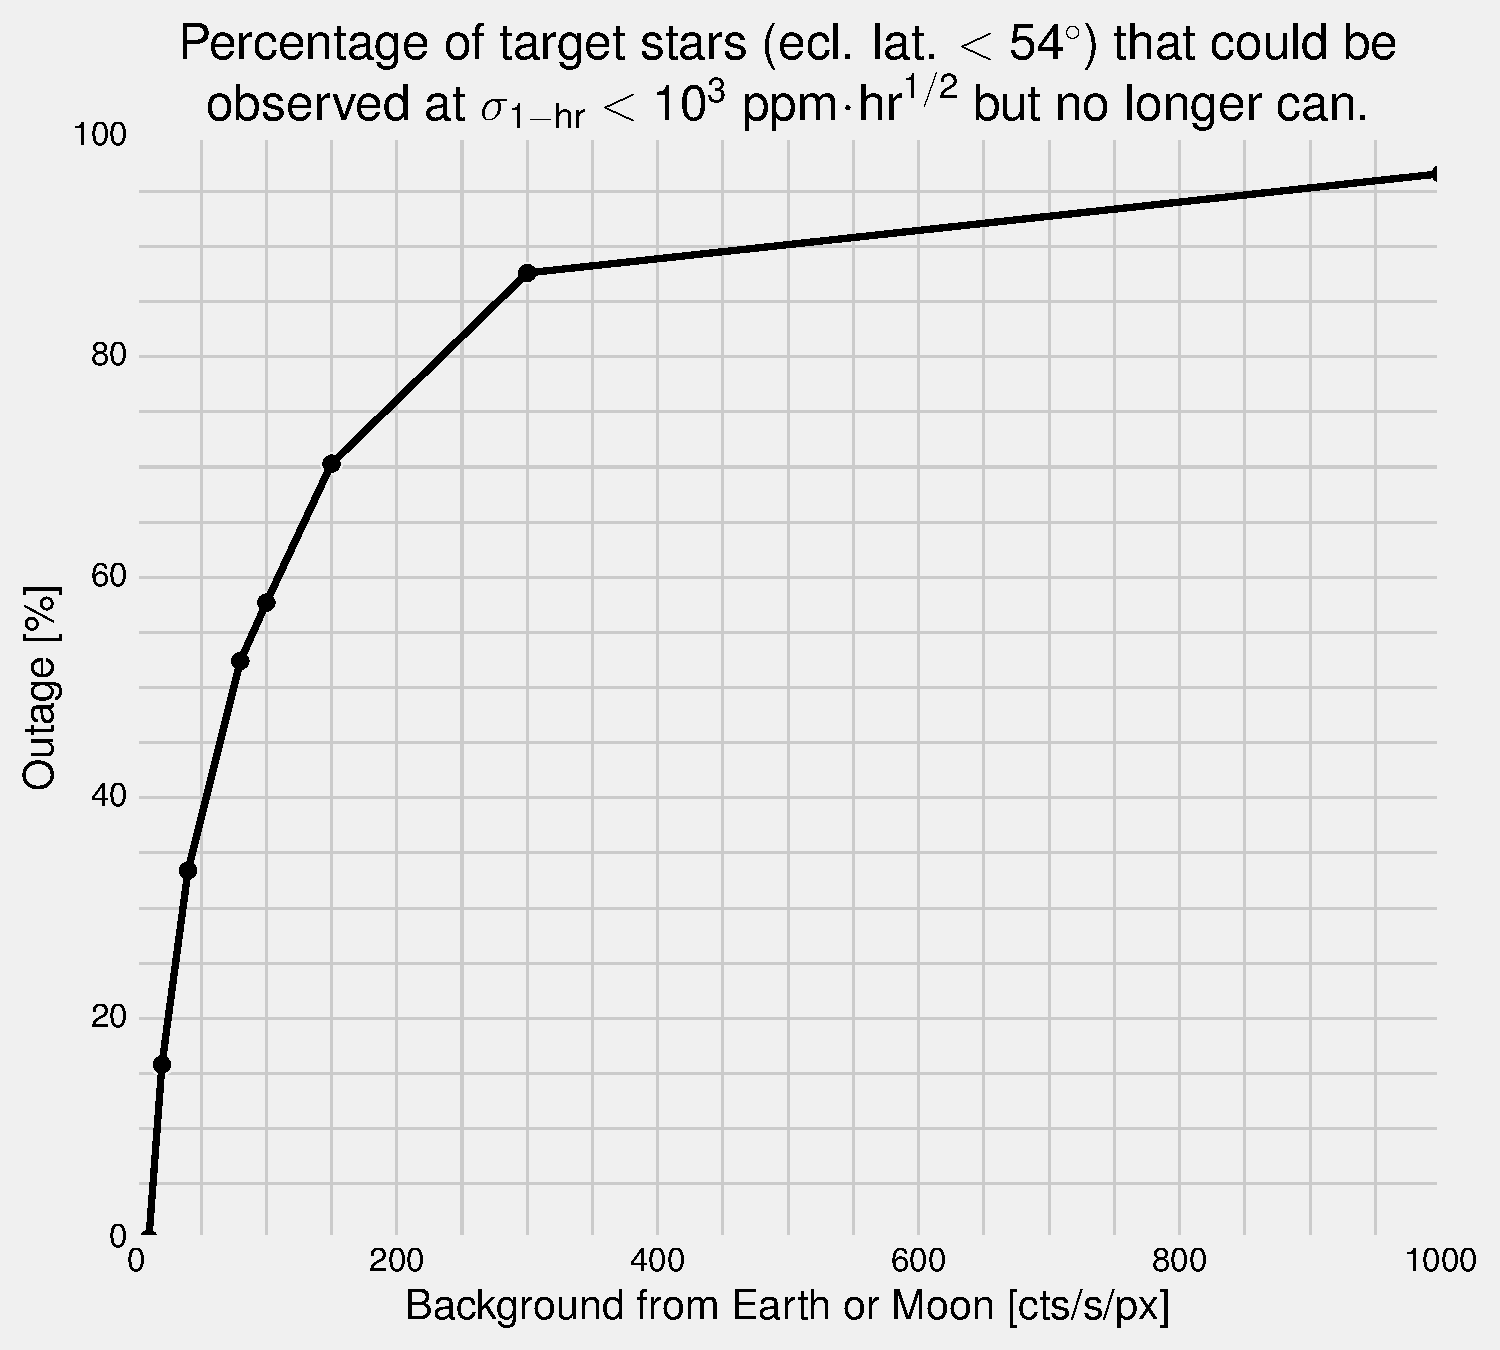
\includegraphics{figures/outage_vs_background.pdf}
	%\missingfigure{foobar}	
	\caption{The procedure described in Sec.~\protect\ref{sec:earth_moon_crossings} drops fields in which $\sim$90\% of the target stars (in the lower two camera fields) cannot be observed.}
	\label{fig:outage_vs_background}
\end{figure*}
\begin{comment}
\section{SNR calculation}
The approach from~\citet{Sullivan_2015} for computing the SNR of any given star is as follows:
\begin{itemize}
	\item Signal is the transit depth for a planet.
	\item Noise sources include photon-counting noise (Poisson shot noise) from the host star and any of its companion stars, zodiacal background shot noise, CCD read noise, and a systematic noise floor of $60\text{ppm}$. Noise from cosmic rays is ignored. 
	The quadrature sum of all these components over a given aperture gives the total noise.
	\item The aperture sizes are found by creating synthetic images of each star with a transiting planet.
	The approach from~\citet{Sullivan_2015} for making these images was:
	\begin{itemize}
		\item Determine the pixel response function (PRF - tells you what fraction of light is collected by a given pixel) based on the star's color and location in the camera field.
		\footnote{This `determination' involves a look-up to the output from a Zemax ray-tracing model of \tesss optics.
		The Zemax model simulates rays passing through the camera optics and into the silicon of the CCD to a probabilistically-determined depth. 
		Excited electrons then diffuse through the remaining depth of the silicon, leading to the PSF.
		We then integrate the PSF over a grid of pixels to arrive at the PRF.}
		\item Sum the PRFs over all wavelengths of incoming light to get a synthetic image of each target star.
	\end{itemize} 
\end{itemize}

The PSFs used by~\citet{Sullivan_2015} were based on idealized assumptions about the camera optics. Laboratory testing of prototype cameras changed some of these assumptions, and led to an `as-built' PSF used in this work which decreases the overall planet yield by $\sim$10-20\%.

Additionally, the approach outlined above has a caveat that was neglected by~\citet{Sullivan_2015}: the PSF, and thus the fraction of stellar flux that will be observed for any given measurement, depends on the position any given target star has on the CCD. 
In other words, for different camera pointings, the quality of \tesss photometry will vary for the same star. 
For instance, the star could land on the corners of the CCD fields, where the shoddier PSF will lead to fewer collected photons and a noiser measurement.
~\citet{Sullivan_2015} dealt with this by taking a running average of the field angles of any given star over the \tess entire mission, and then computing a final PRF and photon flux based on that averaged position.
This is wrong.

We simplified this procedure by saying that `everything lands at the very center of the CCD field, where the PSF is best'.
This \textit{increases} the overall planet yield by $\sim$10-20\%.
\todo{what impact did this have on planet yield? make this discussion better}
\end{comment}

\begin{comment}

\subsection{Population parameters from \nhemi}
\begin{figure*}[t]
	\centering
	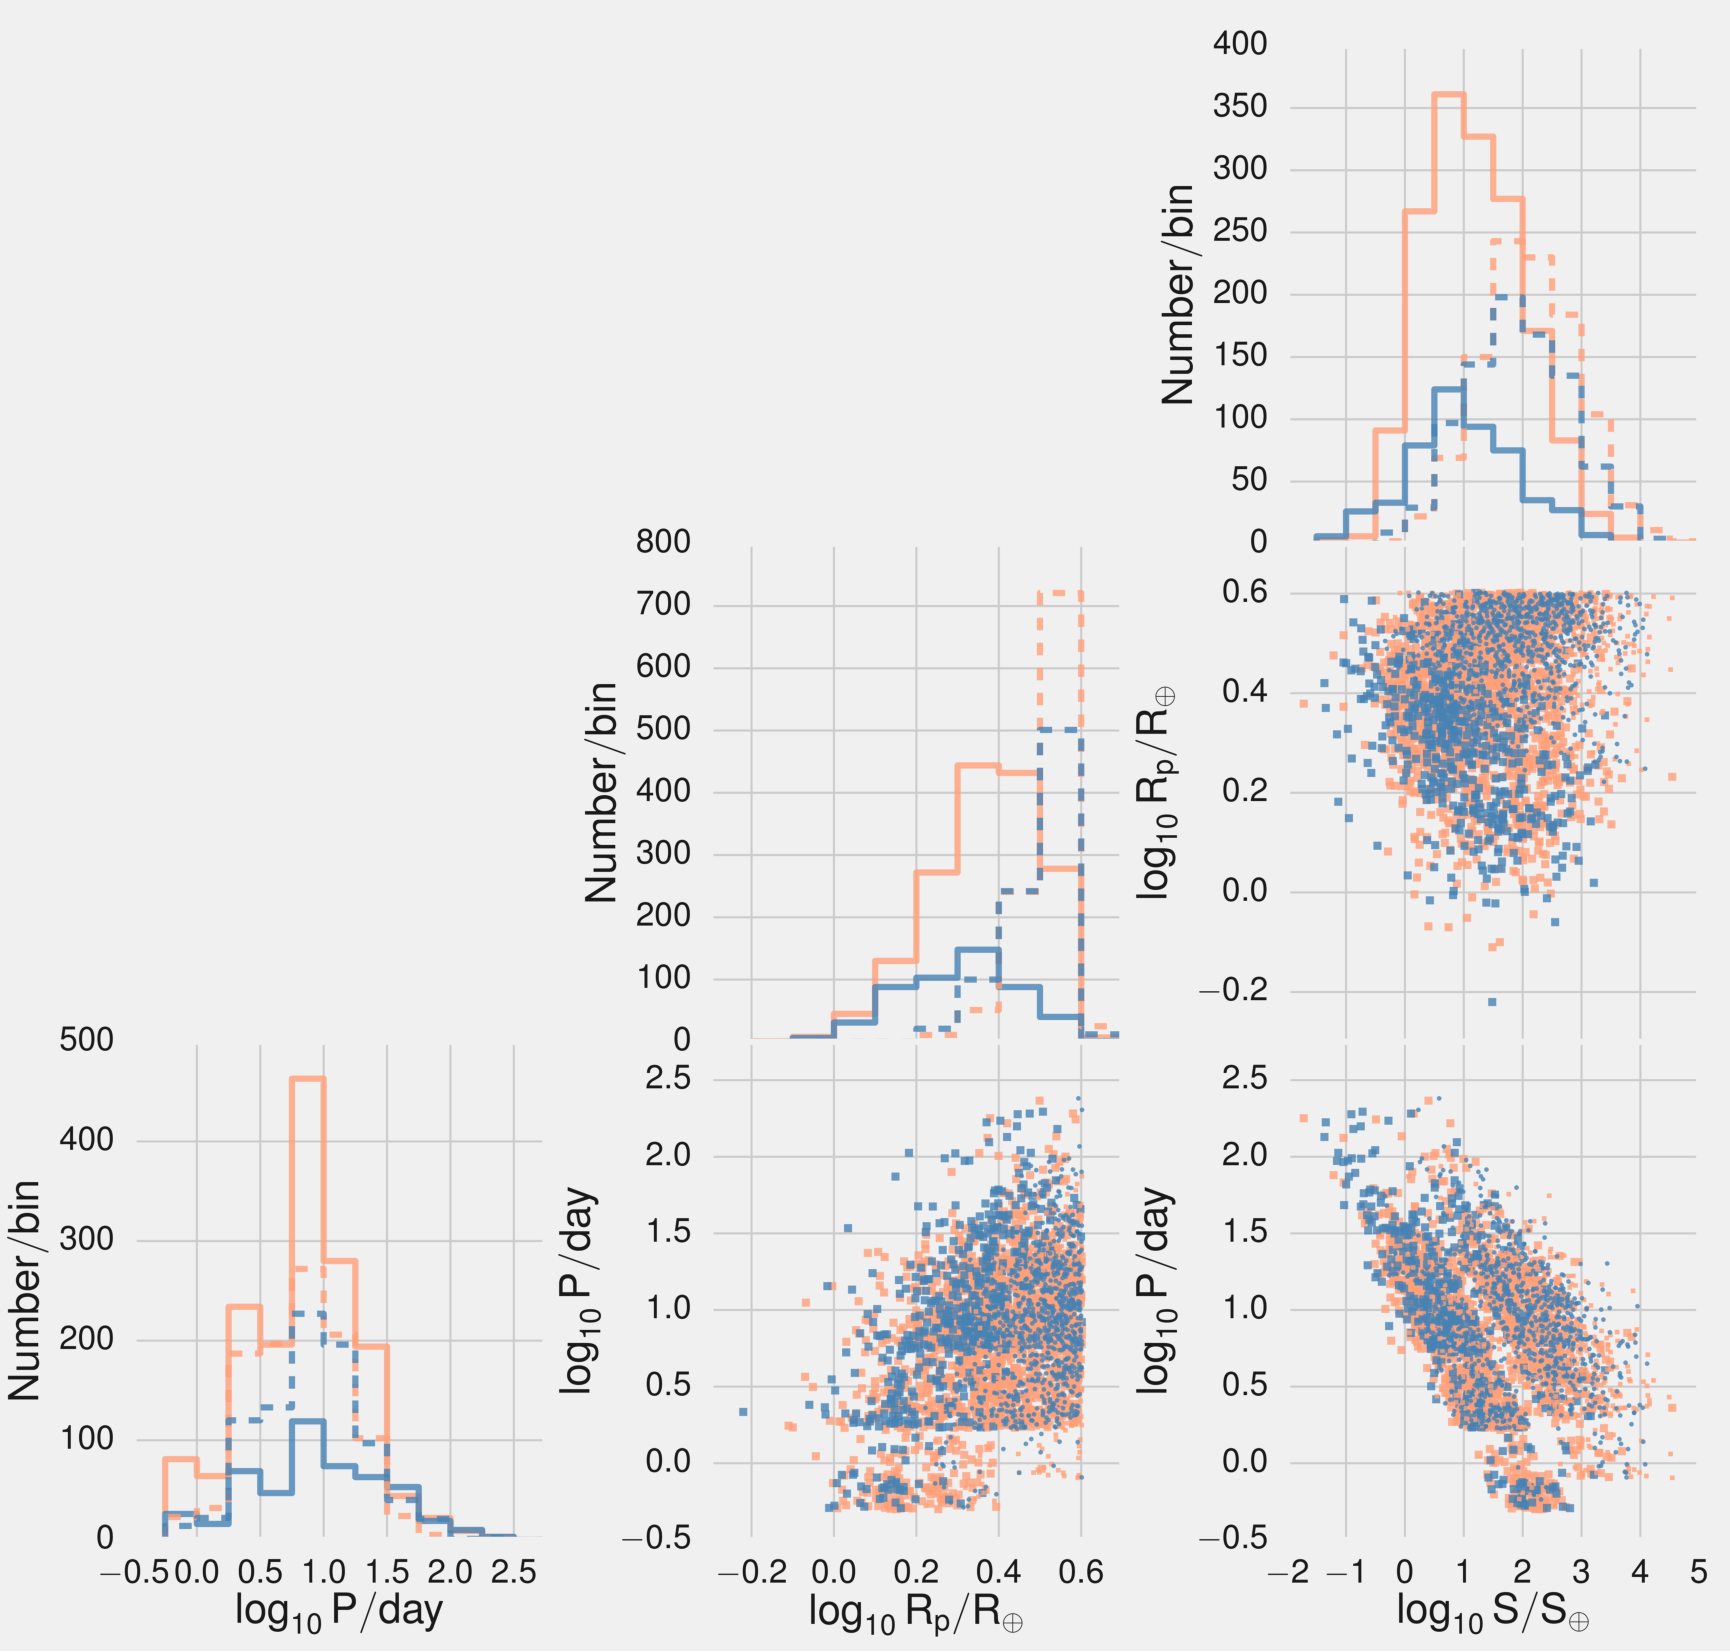
\includegraphics[]{figures/temp_pair_plots_nhemi.pdf}
	\caption{Properties of detected $R<4R_\oplus$ planets from one Monte Carlo realization of the \npole\:scenario. Legend is the same as in Fig.~\protect\ref{fig:imag_vs_teff_nhemi} -- orange: detected in Primary Mission; blue: newly detected from Extended Mission; squares (solid lines): postage stamps; dots (dashed lines): full frame images. We note that $\gg 2\times10^3$ giants ($R > 4R_\oplus$, not shown) should be recoverable from full frame images, but they are not the focus of this work.}
	\label{fig:pair_plots_nhemi}
\end{figure*}
\end{comment}
